\documentclass[landscape]{article}

\usepackage[utf8]{inputenc}
\usepackage[english]{babel}

\usepackage{amsmath,amsfonts,amssymb}
\usepackage{fullpage}
\usepackage{verbatim}

\usepackage[margin=10mm, top=5mm, bottom=5mm]{geometry}

\usepackage{tikz,pgfplots}

\pgfplotsset{
  width=240mm,height=180mm,
  major grid style={thin,dotted,color=black!50},
  minor grid style={thin,dotted,color=black!50},
  grid,
  every axis/.append style={
    line width=1pt,
    tick style={
      line cap=round,
      thin,
      major tick length=4pt,
      minor tick length=2pt,
    },
  },
  legend cell align=left,
  legend pos=north west,
  compat=1.9
}

%%%%%%%%%%%%%%%%%%%%%%%%%%%%%%%%%%%%%%%%%%%%%%%%%%%%%%%%%%%%%%%%%%%%%%%%%%%%%%%%

\begin{document}

% IMPORT-DATA Results Results_muc.txt

\begin{center}

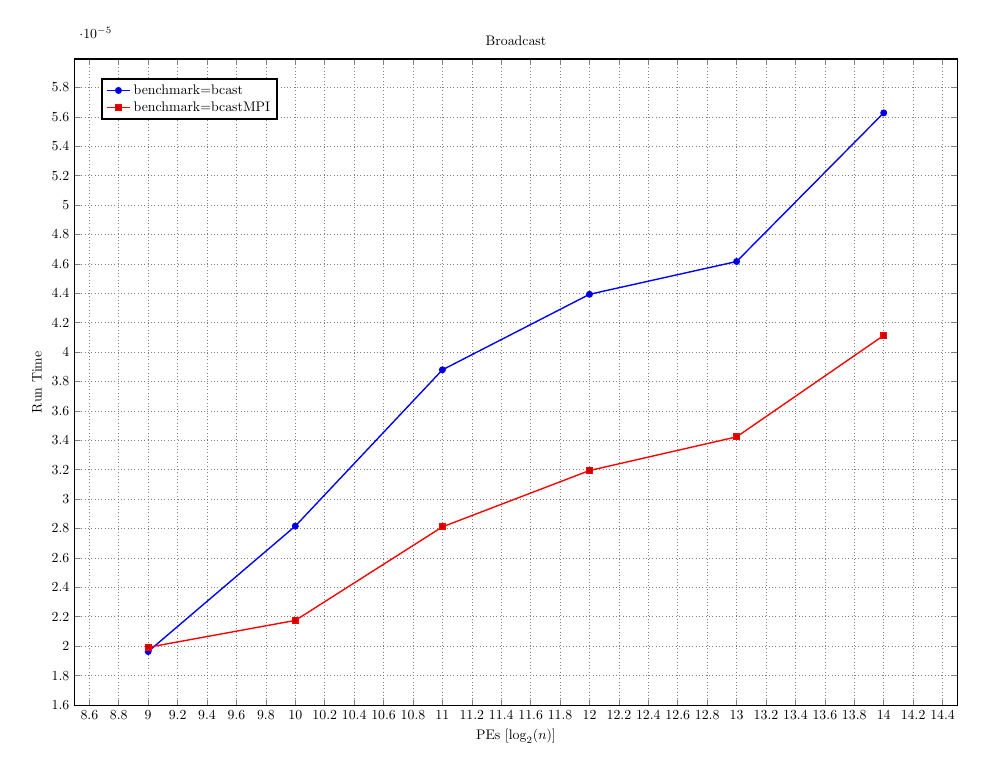
\begin{tikzpicture}  [scale=0.5]
  \begin{axis}[
    title={Broadcast},
    xlabel={PEs [$\log_2(n)$]},
    ylabel={Run Time},
    ]    

    %% MULTIPLOT(benchmark) SELECT LOG(2, size) AS x, MEDIAN(time) AS y, MULTIPLOT
    %% FROM Results 
    %% WHERE iteration>0 AND (benchmark = "bcast" OR benchmark = "bcastMPI")
    %% GROUP BY MULTIPLOT, x  ORDER BY MULTIPLOT, x
    \addplot coordinates { (9.0,1.96323e-05) (10.0,2.81623e-05) (11.0,3.87914e-05) (12.0,4.39286e-05) (13.0,4.61582e-05) (14.0,5.62668e-05) };
    \addlegendentry{benchmark=bcast};
    \addplot coordinates { (9.0,1.9921e-05) (10.0,2.17482e-05) (11.0,2.81129e-05) (12.0,3.19425e-05) (13.0,3.42317e-05) (14.0,4.11309e-05) };
    \addlegendentry{benchmark=bcastMPI};

  \end{axis}
\end{tikzpicture}
\newpage

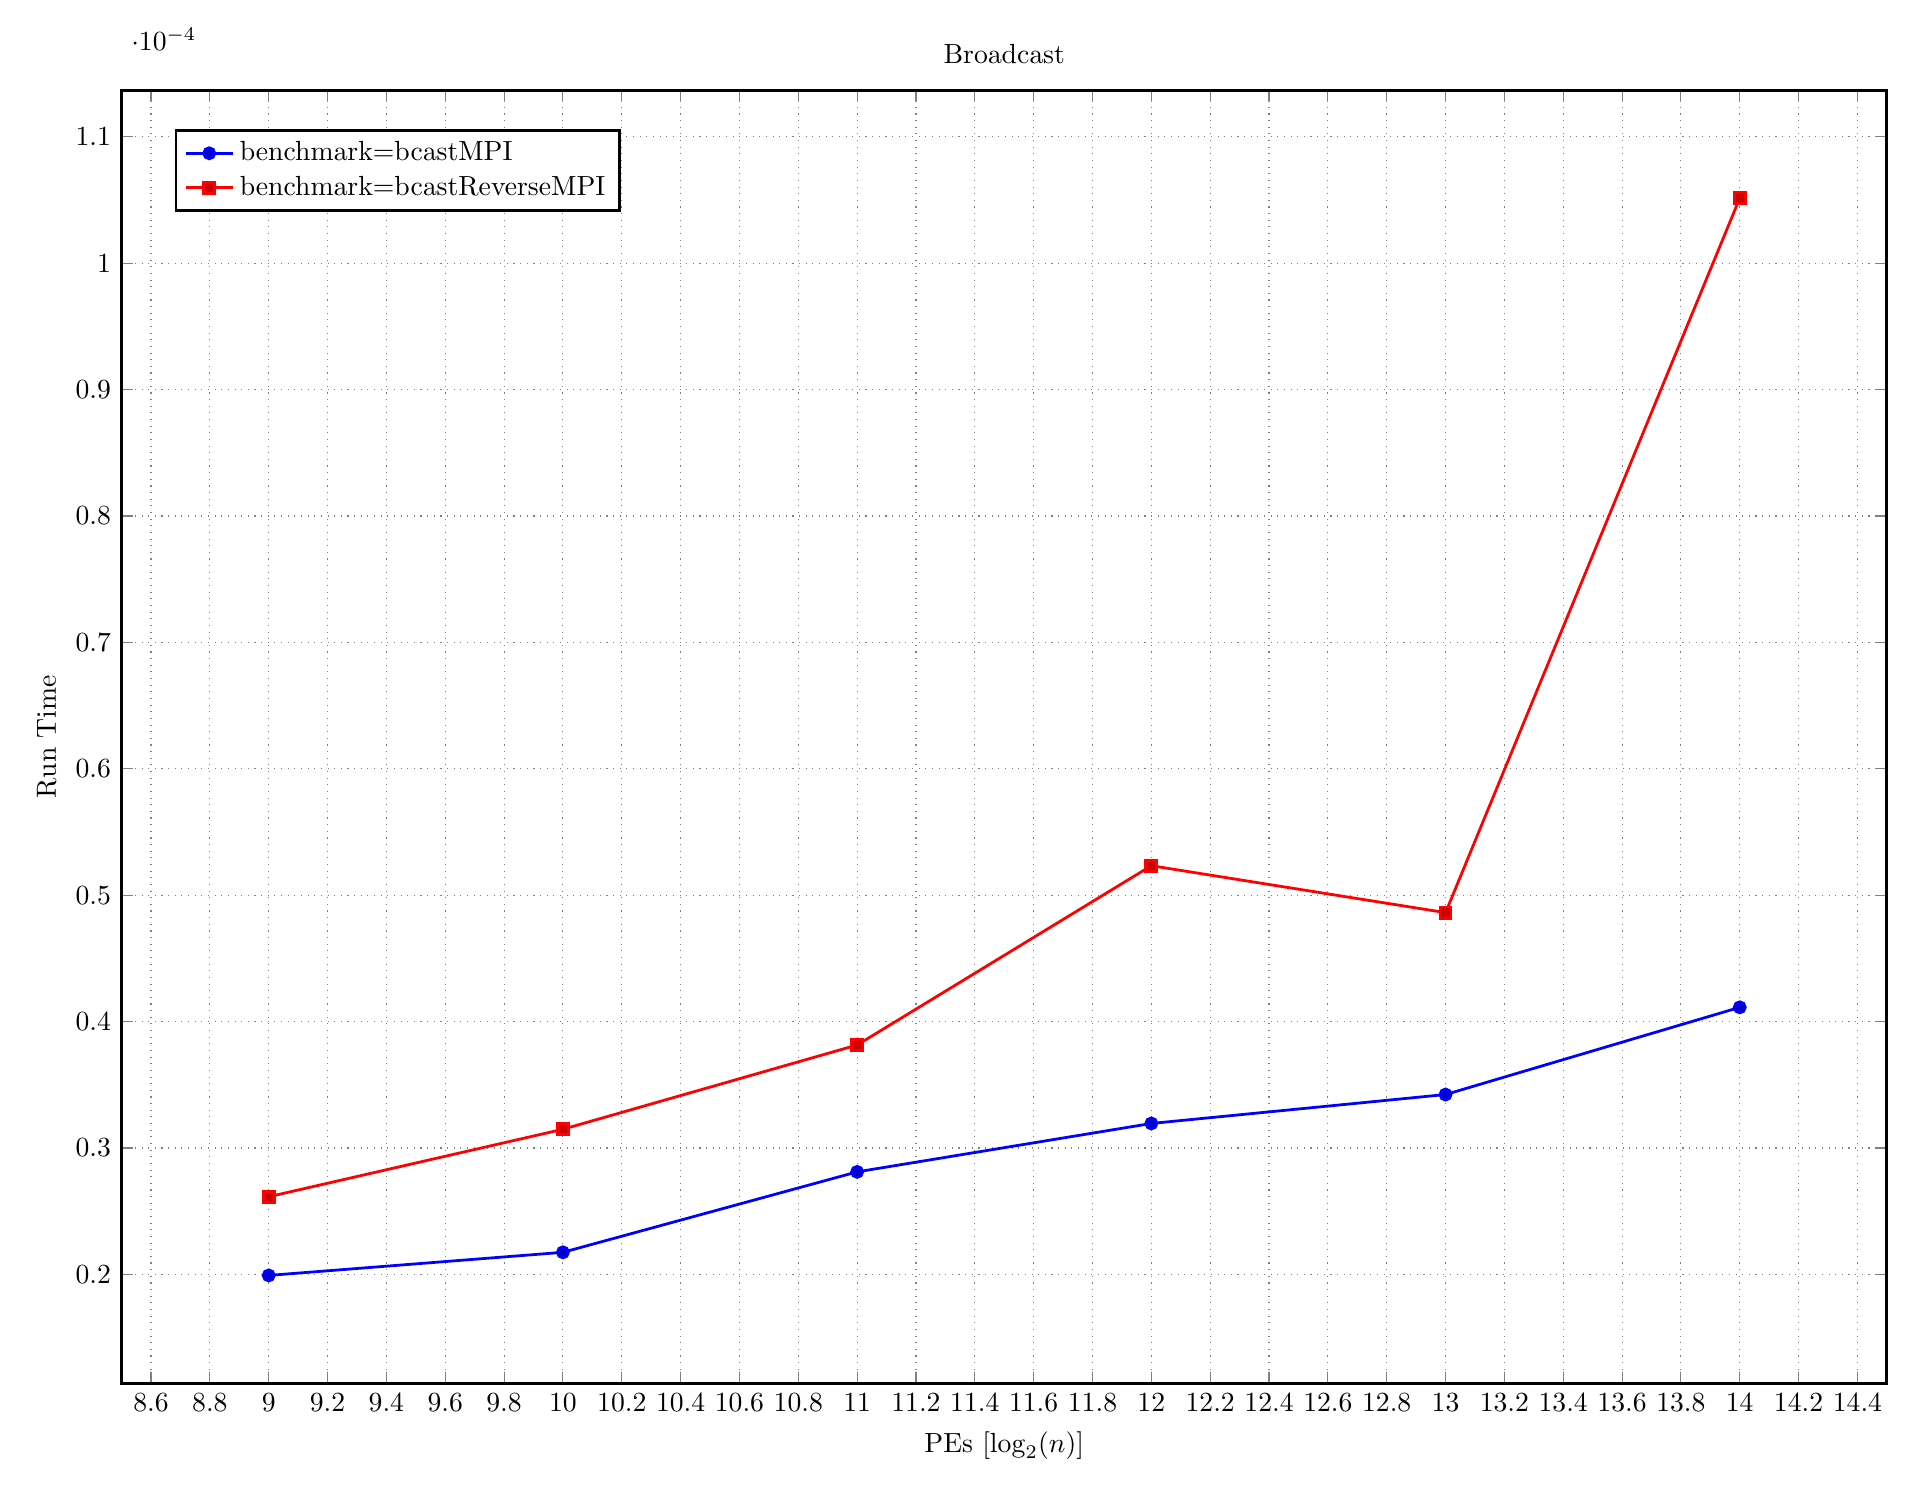
\begin{tikzpicture}
  \begin{axis}[
    title={Broadcast},
    xlabel={PEs [$\log_2(n)$]},
    ylabel={Run Time},
    ]

    %% MULTIPLOT(benchmark) SELECT LOG(2, size) AS x, MEDIAN(time) AS y, MULTIPLOT
    %% FROM Results 
    %% WHERE iteration>0 AND (benchmark = "bcastMPI" OR benchmark="bcastReverse" OR benchmark="bcastReverseMPI")
    %% GROUP BY MULTIPLOT, x  ORDER BY MULTIPLOT, x
    \addplot coordinates { (9.0,1.9921e-05) (10.0,2.17482e-05) (11.0,2.81129e-05) (12.0,3.19425e-05) (13.0,3.42317e-05) (14.0,4.11309e-05) };
    \addlegendentry{benchmark=bcastMPI};
    \addplot coordinates { (9.0,2.61441e-05) (10.0,3.14843e-05) (11.0,3.81507e-05) (12.0,5.23347e-05) (13.0,4.86225e-05) (14.0,0.000105152) };
    \addlegendentry{benchmark=bcastReverseMPI};

  \end{axis}
\end{tikzpicture}
\newpage

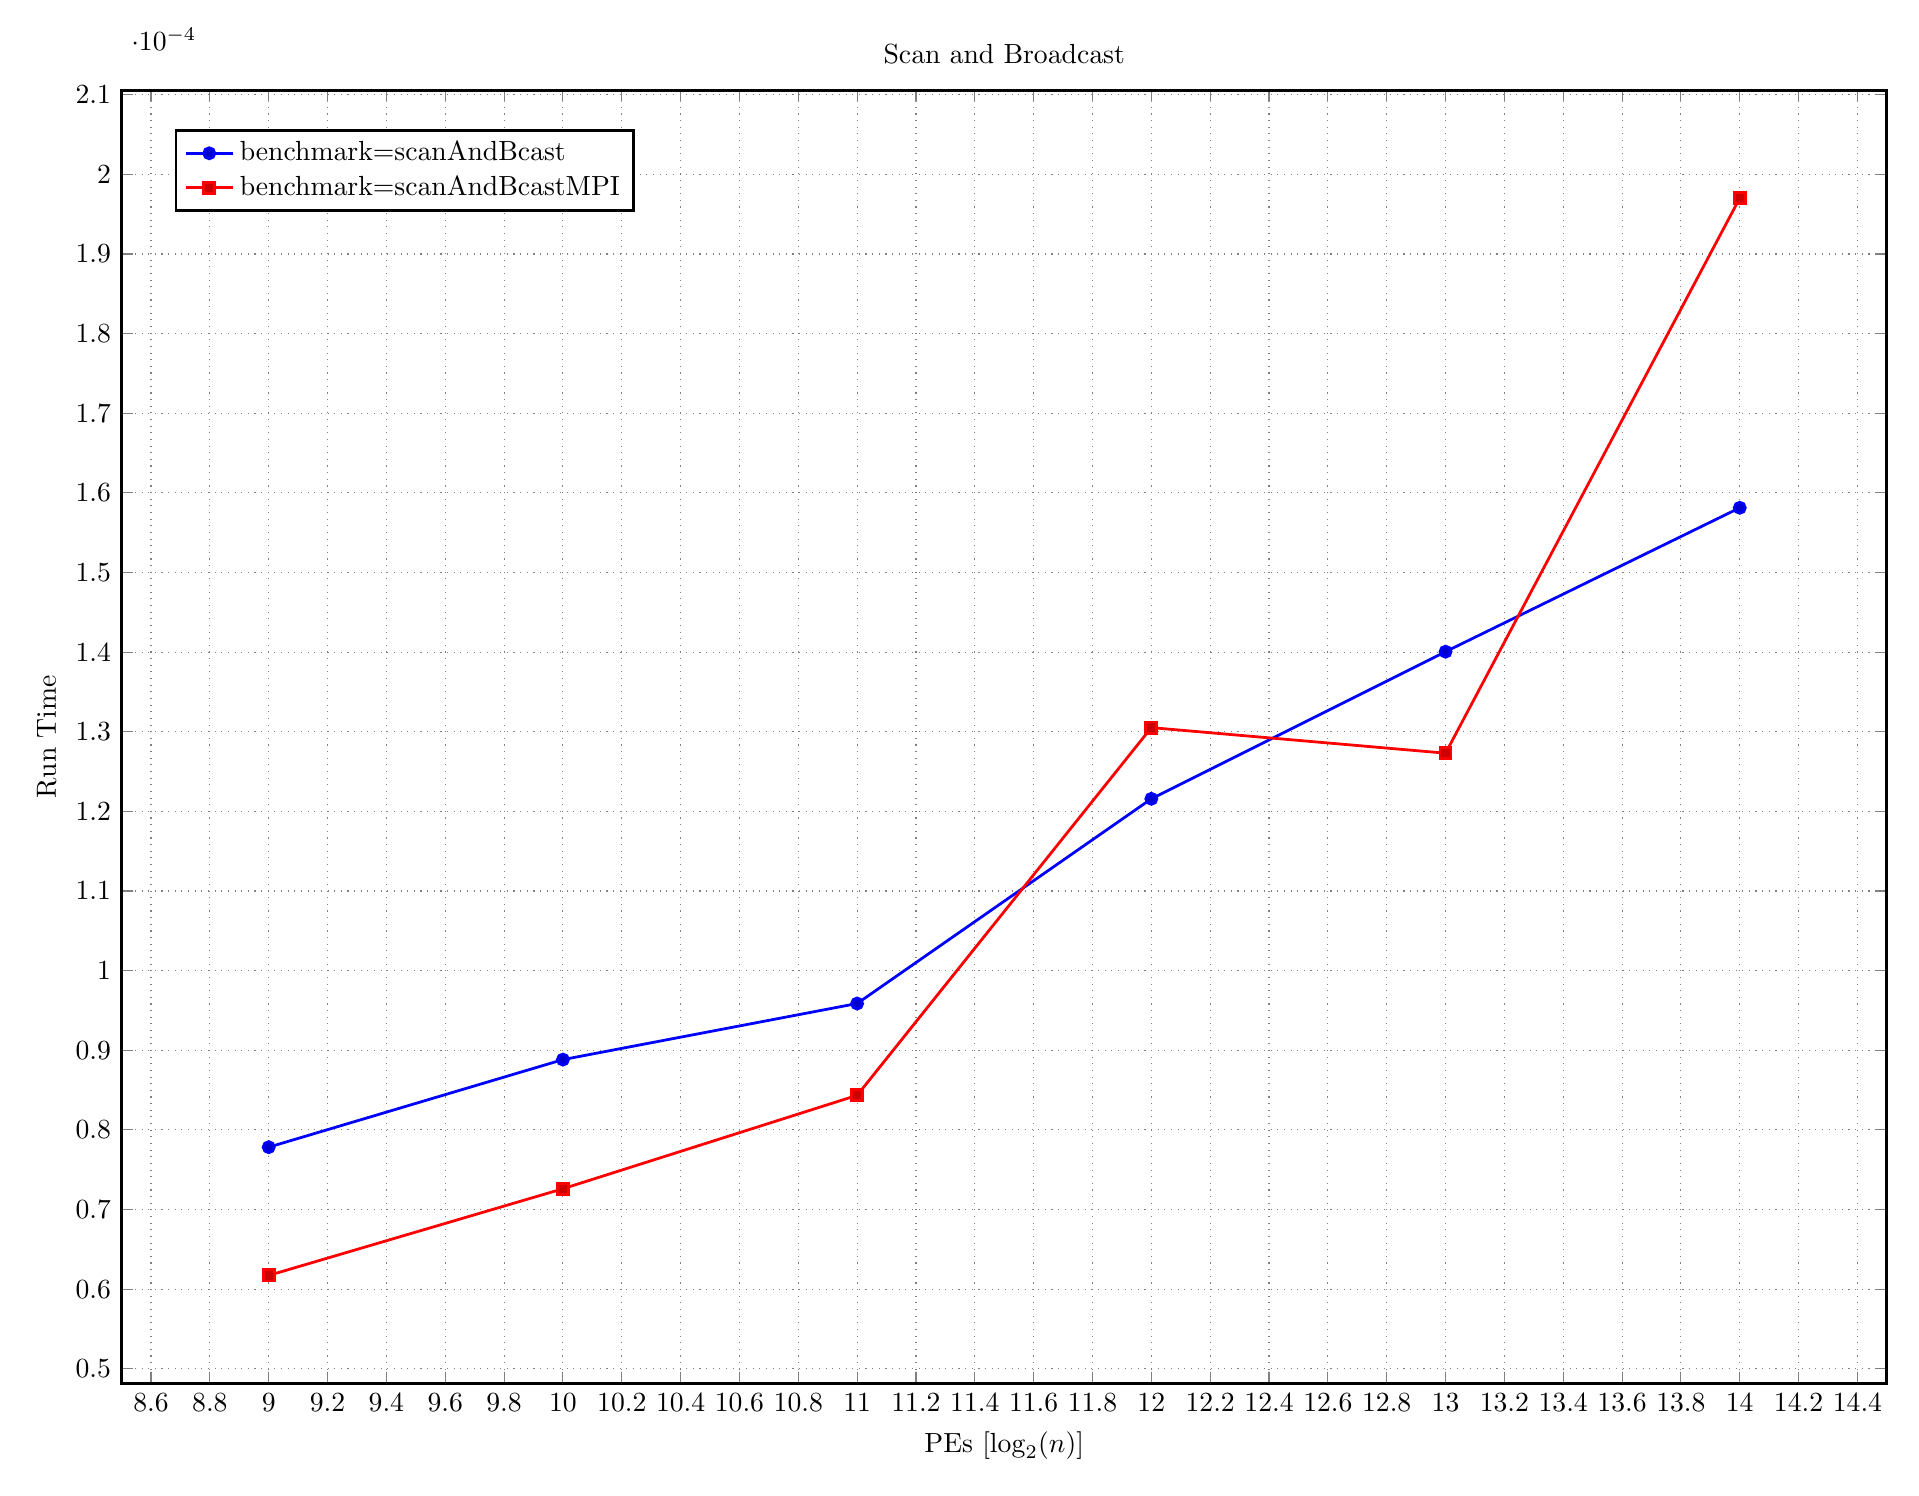
\begin{tikzpicture}
  \begin{axis}[
    title={Scan and Broadcast},
    xlabel={PEs [$\log_2(n)$]},
    ylabel={Run Time},
    ]

    %% MULTIPLOT(benchmark) SELECT LOG(2, size) AS x, MEDIAN(time) AS y, MULTIPLOT
    %% FROM Results
    %% WHERE iteration>0 AND (benchmark = "scanAndBcast" OR benchmark = "scanAndBcastMPI")
    %% GROUP BY MULTIPLOT, x  ORDER BY MULTIPLOT, x
    \addplot coordinates { (9.0,7.78269e-05) (10.0,8.8824e-05) (11.0,9.58666e-05) (12.0,0.000121575) (13.0,0.000140052) (14.0,0.000158124) };
    \addlegendentry{benchmark=scanAndBcast};
    \addplot coordinates { (9.0,6.17206e-05) (10.0,7.2604e-05) (11.0,8.43368e-05) (12.0,0.000130514) (13.0,0.000127304) (14.0,0.000197016) };
    \addlegendentry{benchmark=scanAndBcastMPI};

  \end{axis}
\end{tikzpicture}
\newpage

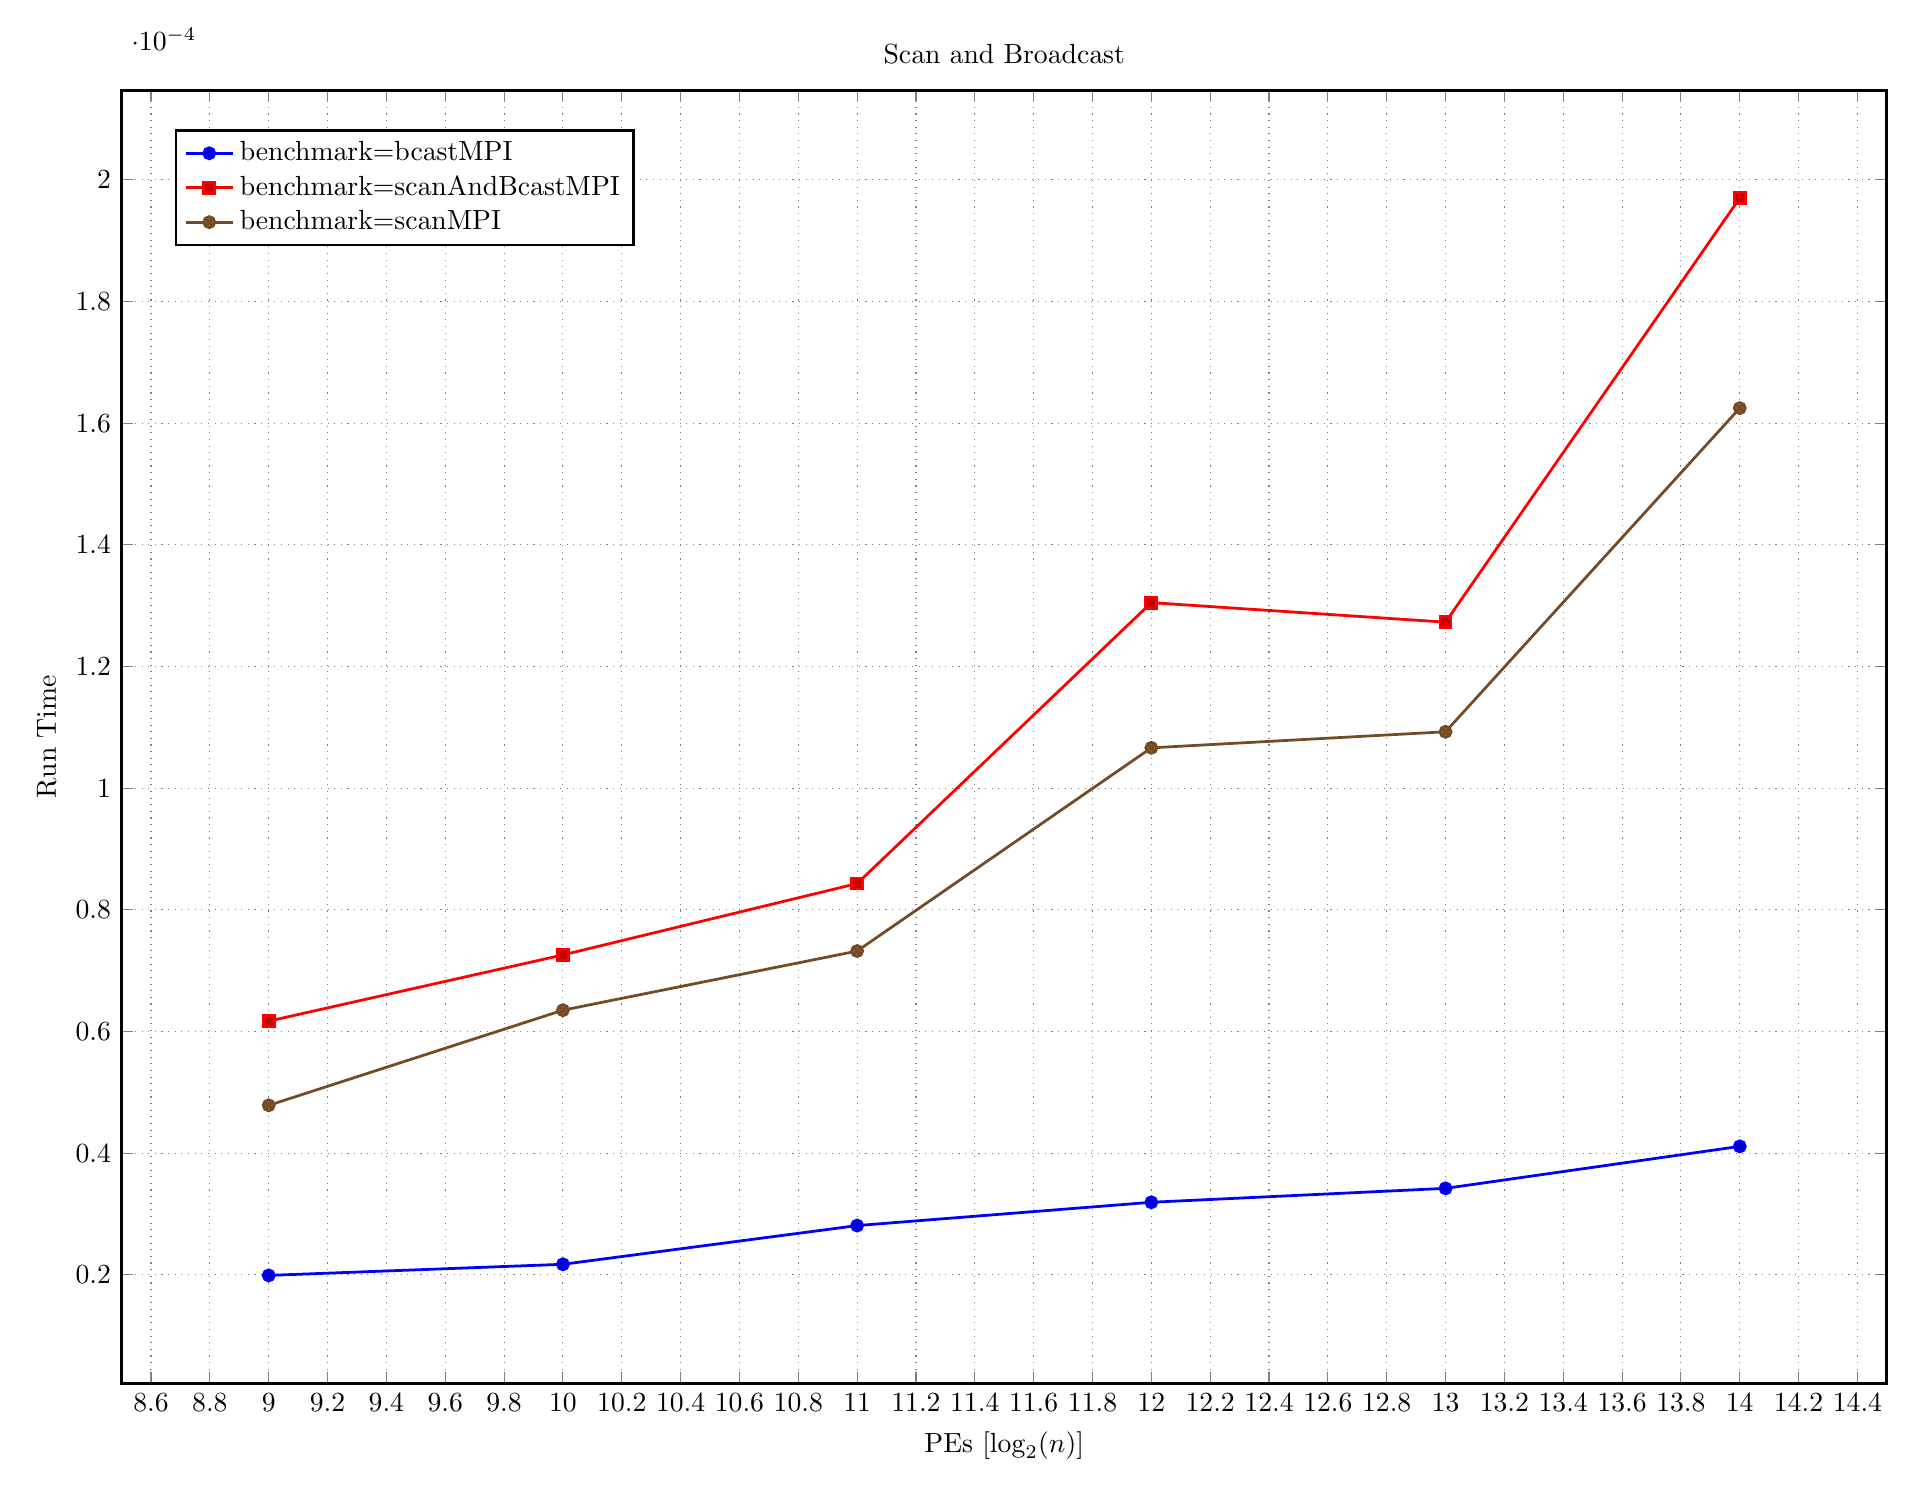
\begin{tikzpicture}
  \begin{axis}[
    title={Scan and Broadcast},
    xlabel={PEs [$\log_2(n)$]},
    ylabel={Run Time},
    ]

    %% MULTIPLOT(benchmark) SELECT LOG(2, size) AS x, MEDIAN(time) AS y, MULTIPLOT
    %% FROM Results
    %% WHERE iteration>0 AND (benchmark = "scanAndBcastMPI" OR benchmark = "scanMPI" OR benchmark="bcastMPI") 
    %% GROUP BY MULTIPLOT, x  ORDER BY MULTIPLOT, x
    \addplot coordinates { (9.0,1.9921e-05) (10.0,2.17482e-05) (11.0,2.81129e-05) (12.0,3.19425e-05) (13.0,3.42317e-05) (14.0,4.11309e-05) };
    \addlegendentry{benchmark=bcastMPI};
    \addplot coordinates { (9.0,6.17206e-05) (10.0,7.2604e-05) (11.0,8.43368e-05) (12.0,0.000130514) (13.0,0.000127304) (14.0,0.000197016) };
    \addlegendentry{benchmark=scanAndBcastMPI};
    \addplot coordinates { (9.0,4.78793e-05) (10.0,6.35181e-05) (11.0,7.32429e-05) (12.0,0.000106649) (13.0,0.000109287) (14.0,0.000162488) };
    \addlegendentry{benchmark=scanMPI};

  \end{axis}
\end{tikzpicture}
\newpage

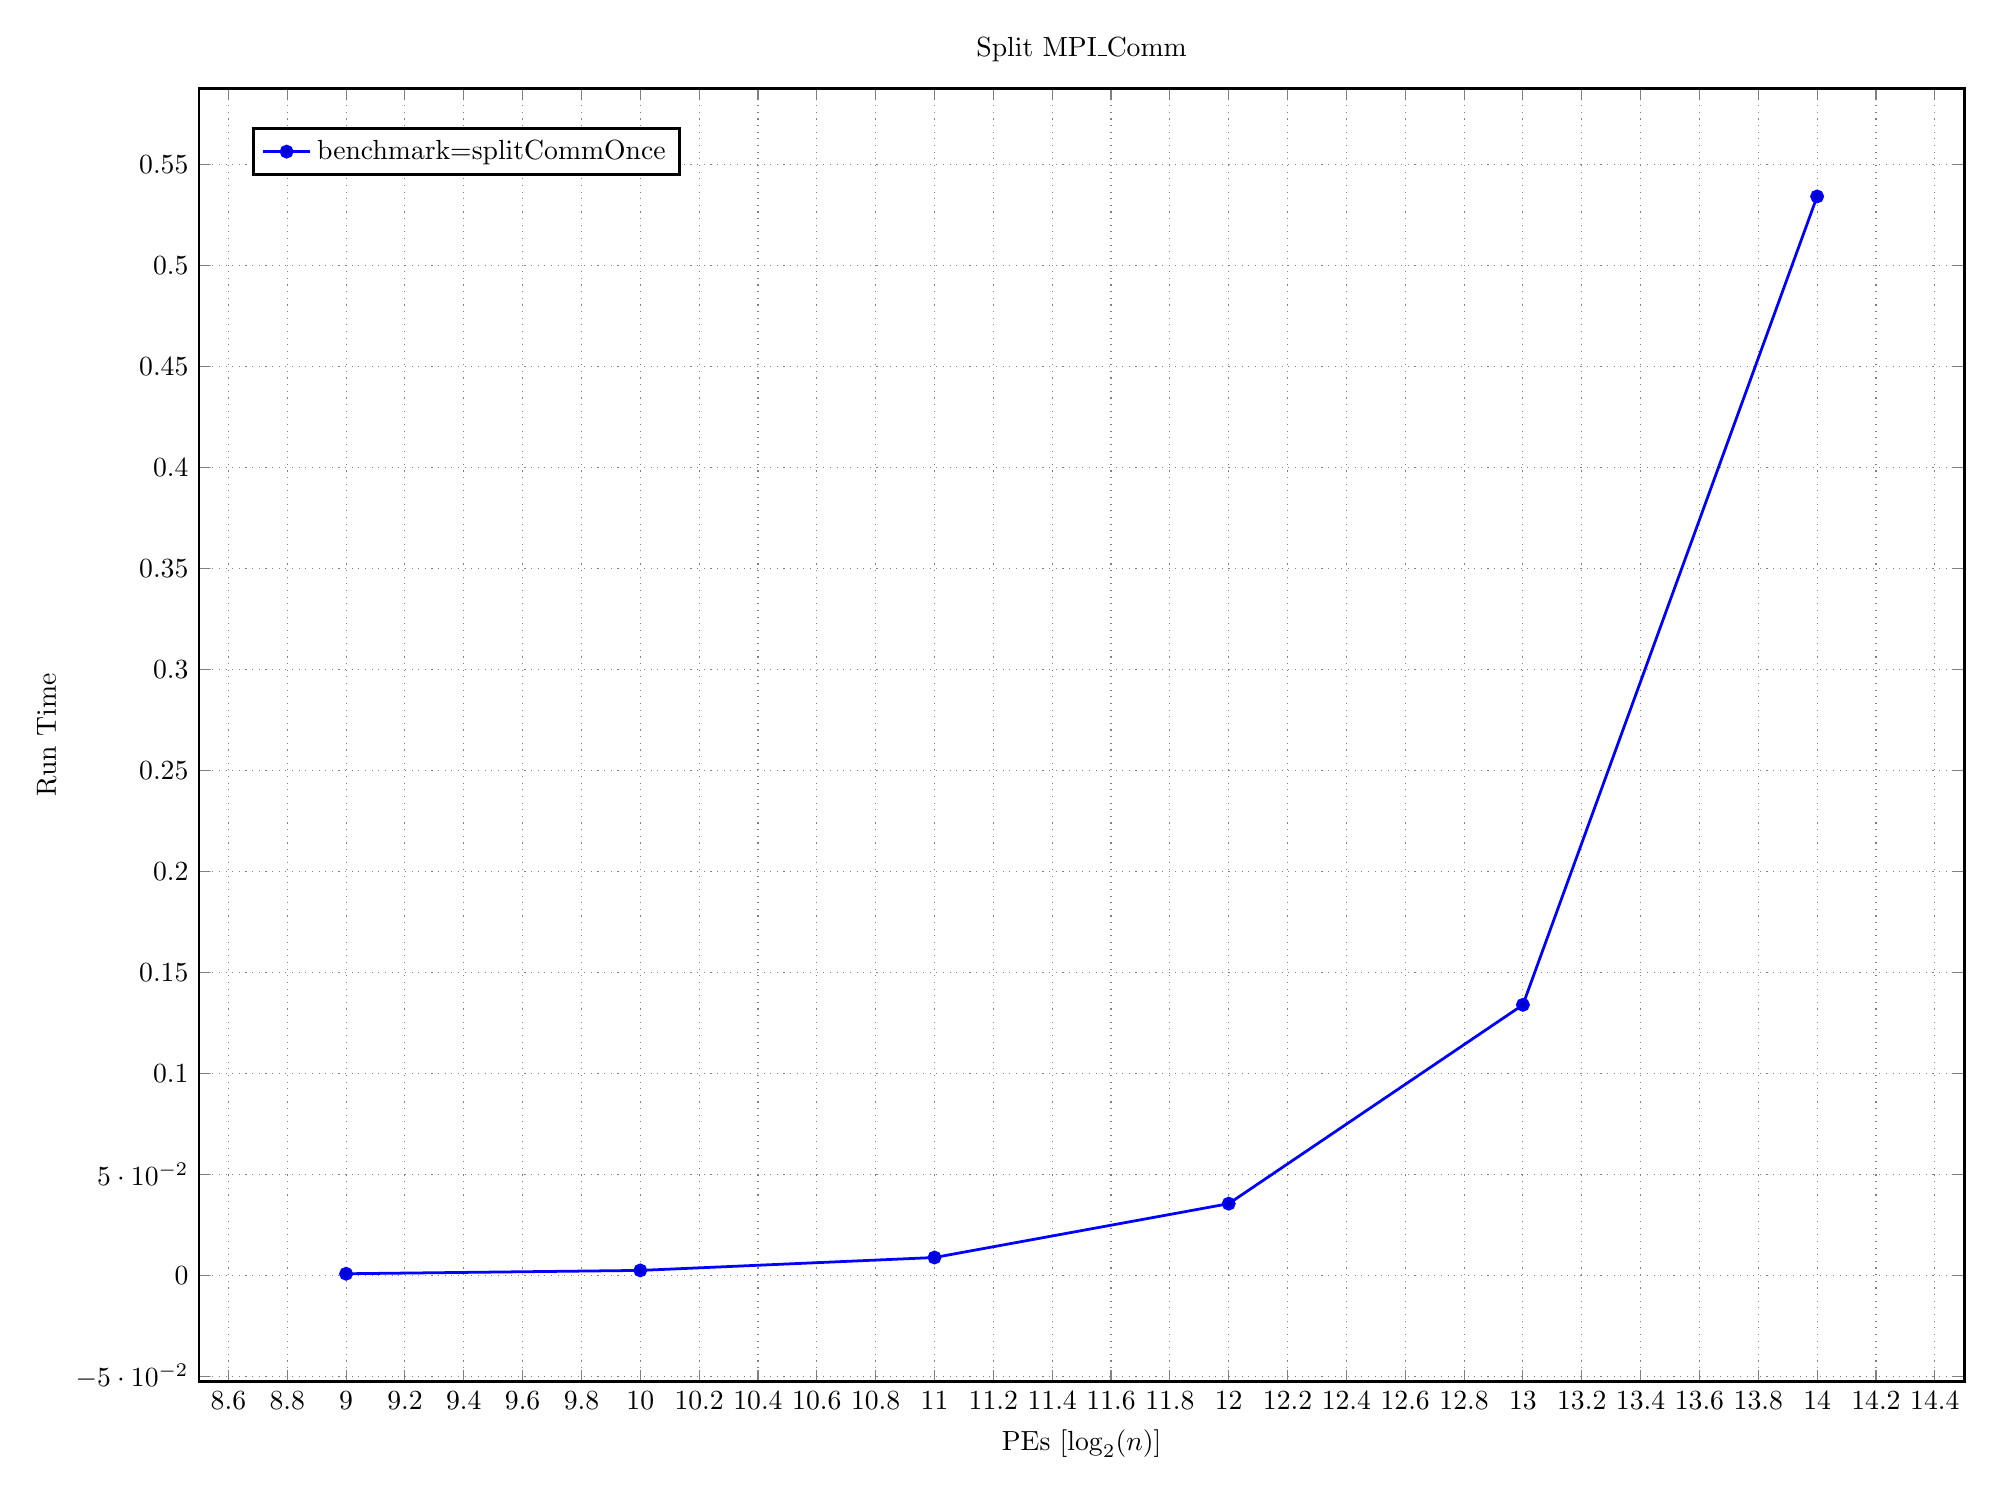
\begin{tikzpicture}
\begin{axis}[
title={Split MPI\_Comm},
xlabel={PEs [$\log_2(n)$]},
ylabel={Run Time},
]

%% MULTIPLOT(benchmark) SELECT LOG(2, size) AS x, MEDIAN(time) AS y, MULTIPLOT
%% FROM Results
%% WHERE iteration>0 AND benchmark = "splitCommOnce"
%% GROUP BY MULTIPLOT, x  ORDER BY MULTIPLOT, x
\addplot coordinates { (9.0,0.0006862) (10.0,0.00233685) (11.0,0.00873223) (12.0,0.0353889) (13.0,0.133876) (14.0,0.534246) };
\addlegendentry{benchmark=splitCommOnce};

\end{axis}
\end{tikzpicture}
\newpage

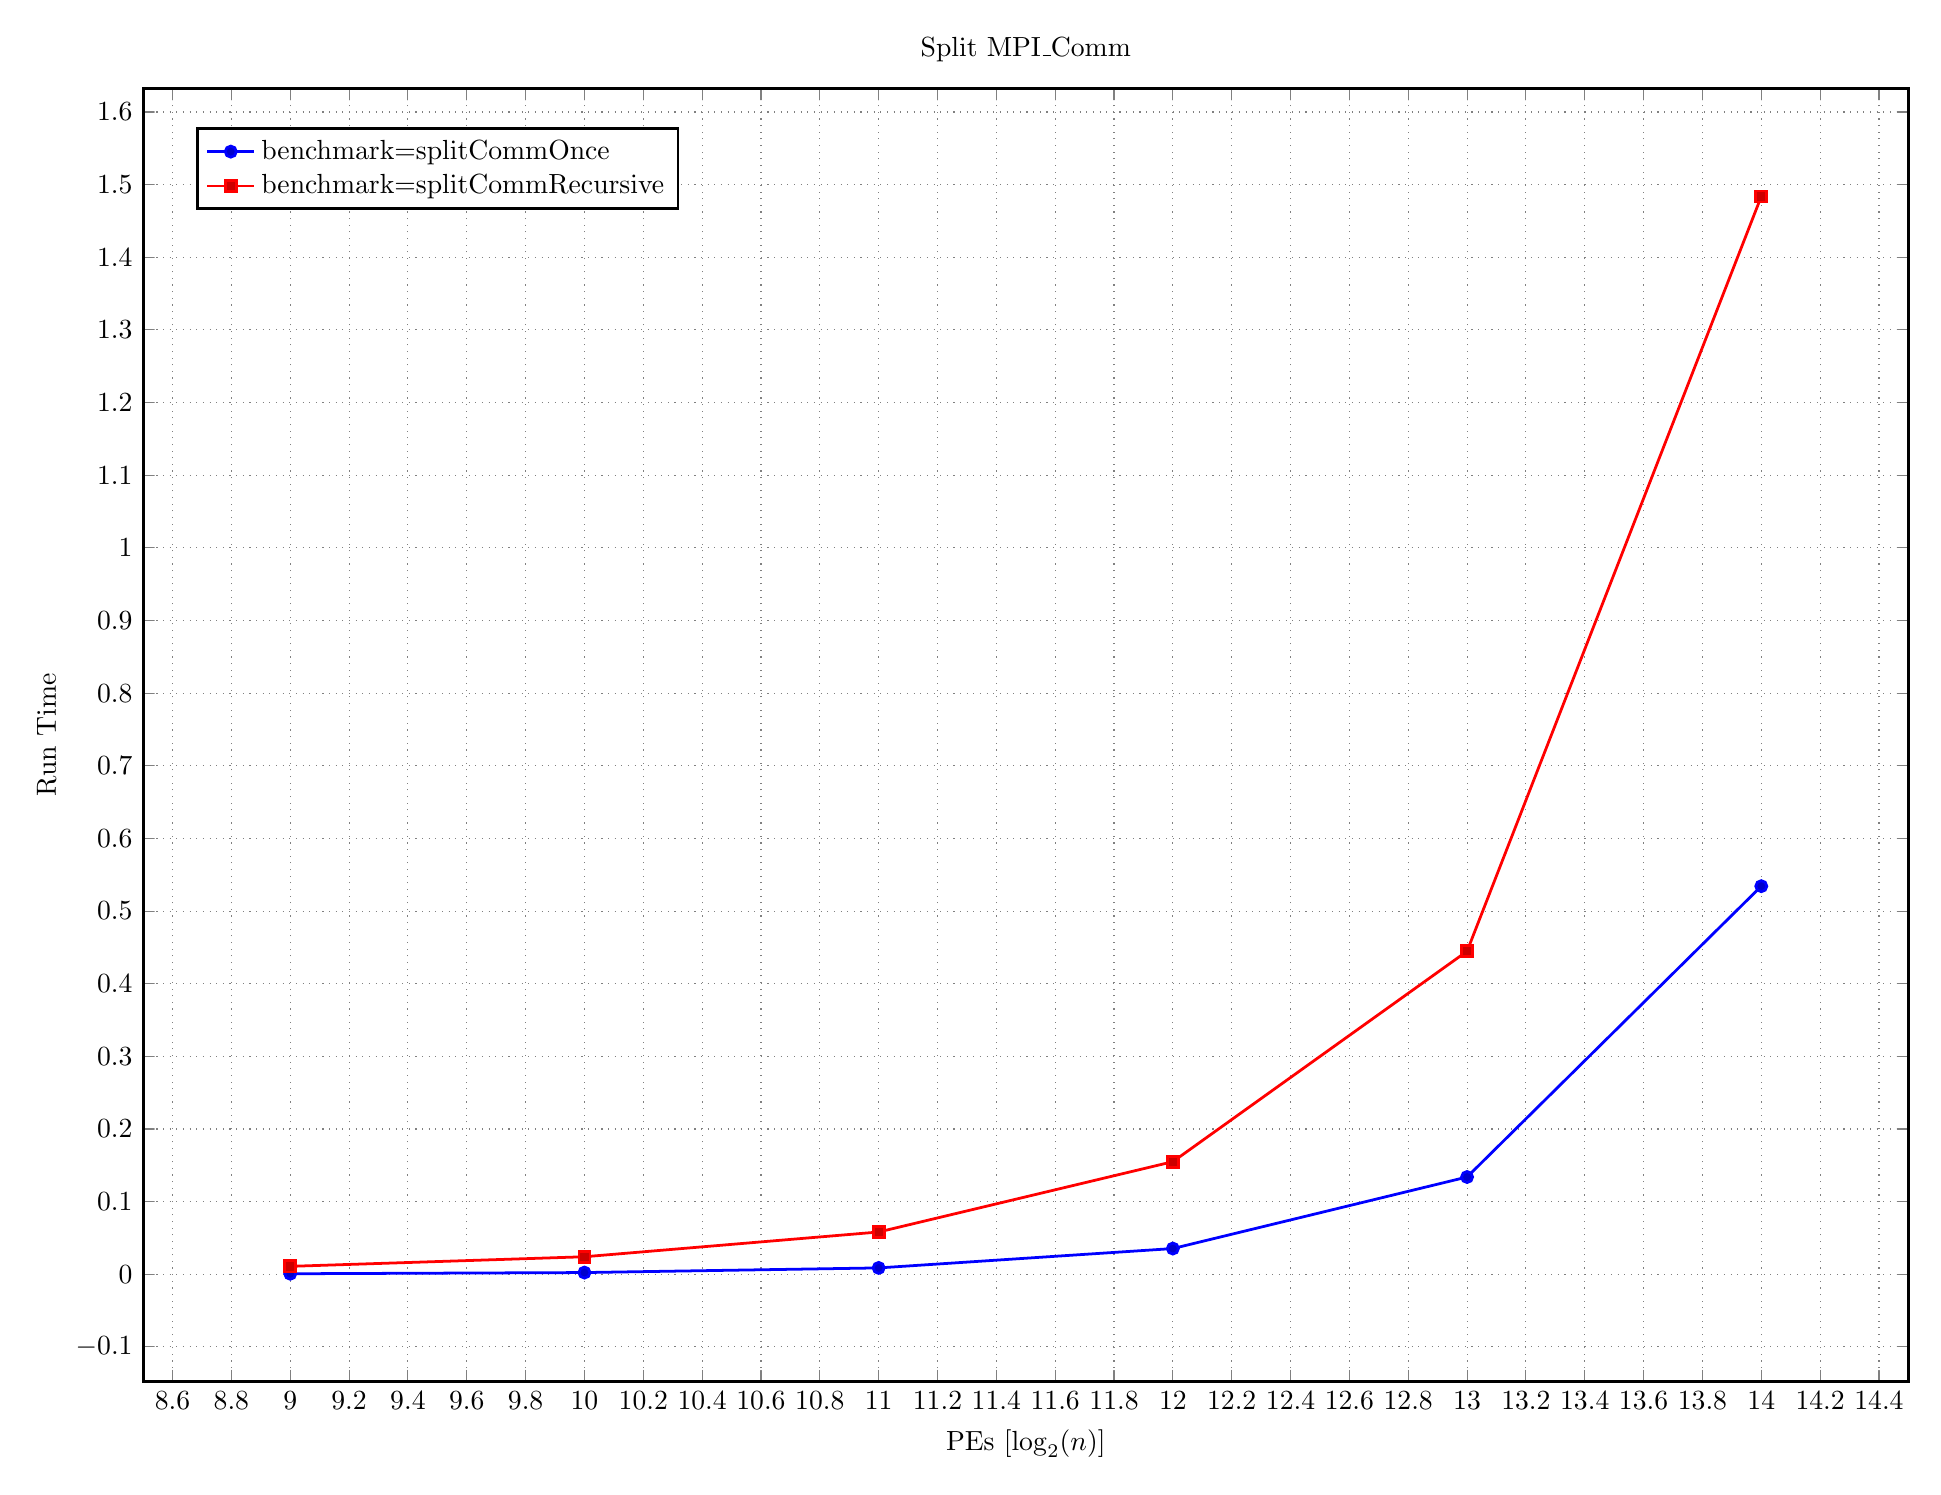
\begin{tikzpicture}
  \begin{axis}[
    title={Split MPI\_Comm},
    xlabel={PEs [$\log_2(n)$]},
    ylabel={Run Time},
    ]

    %% MULTIPLOT(benchmark) SELECT LOG(2, size) AS x, MEDIAN(time) AS y, MULTIPLOT
    %% FROM Results
    %% WHERE iteration>0 AND (benchmark = "splitCommOnce" OR benchmark="splitCommRecursive")
    %% GROUP BY MULTIPLOT, x  ORDER BY MULTIPLOT, x
    \addplot coordinates { (9.0,0.0006862) (10.0,0.00233685) (11.0,0.00873223) (12.0,0.0353889) (13.0,0.133876) (14.0,0.534246) };
    \addlegendentry{benchmark=splitCommOnce};
    \addplot coordinates { (9.0,0.0108791) (10.0,0.0240967) (11.0,0.0581707) (12.0,0.154987) (13.0,0.444716) (14.0,1.48378) };
    \addlegendentry{benchmark=splitCommRecursive};

  \end{axis}
\end{tikzpicture}
\newpage

\begin{table}\centering
\begin{tabular}{l|rrrr}
	$n$ & splitCommOnce & splitCommRec & scanAndBcastMPI & bcast \\ \hline
	%% TABULAR REFORMAT(col 1-4=(precision=2))
	%% SELECT '$2^{' || FLOOR(LOG(2, size)) || '}$',
	%% (SELECT AVG(time)*1000 FROM Results s1 WHERE s1.benchmark='splitCommOnce' AND s1.size = s.size GROUP BY s1.size),
	%% (SELECT AVG(time)*1000 FROM Results s1 WHERE s1.benchmark='splitCommRecursive' AND s1.size = s.size GROUP BY s1.size),
	%% (SELECT AVG(time)*1000 FROM Results s1 WHERE s1.benchmark='scanAndBcastMPI' AND s1.size = s.size GROUP BY s1.size),
	%% (SELECT AVG(time)*1000 FROM Results s1 WHERE s1.benchmark='bcast' AND s1.size = s.size GROUP BY 	s1.size)
	%% FROM Results s
	%% GROUP BY s.size ORDER BY s.size
  $2^{9}$ &   0.70 &   13.03 & 0.06 & 0.03 \\
 $2^{10}$ &   2.48 &   26.26 & 0.08 & 0.05 \\
 $2^{11}$ &   8.81 &   60.46 & 0.08 & 0.08 \\
 $2^{12}$ &  39.84 &  157.85 & 0.28 & 0.07 \\
 $2^{13}$ & 136.86 &  449.02 & 0.14 & 0.10 \\
 $2^{14}$ & 581.65 & 1609.93 & 0.21 & 0.11 \\
 % END TABULAR SELECT '$2^{' || FLOOR(LOG(2, size)) || '}$', (SELECT AVG(time)...
\end{tabular}
\caption{Runtime in $10^{-3}$ s}
\end{table}

\end{center}

\end{document}

%%%%%%%%%%%%%%%%%%%%%%%%%%%%%%%%%%%%%%%%%%%%%%%%%%%%%%%%%%%%%%%%%%%%%%%%%%%%%%%%
